\subsection{Main Landing Pages}
\noindent
When a farmer user or agronomist user logs into their account from the mobile-friendly web application as shown in Figure \ref{fig:mock_login}, they will land on their associated homepages as shown in Figures \ref{fig:mock_farmer} and \ref{fig:mock_agronomist}, respectively. 

\begin{multicols}{3}
\begin{figure}[H]
\centering
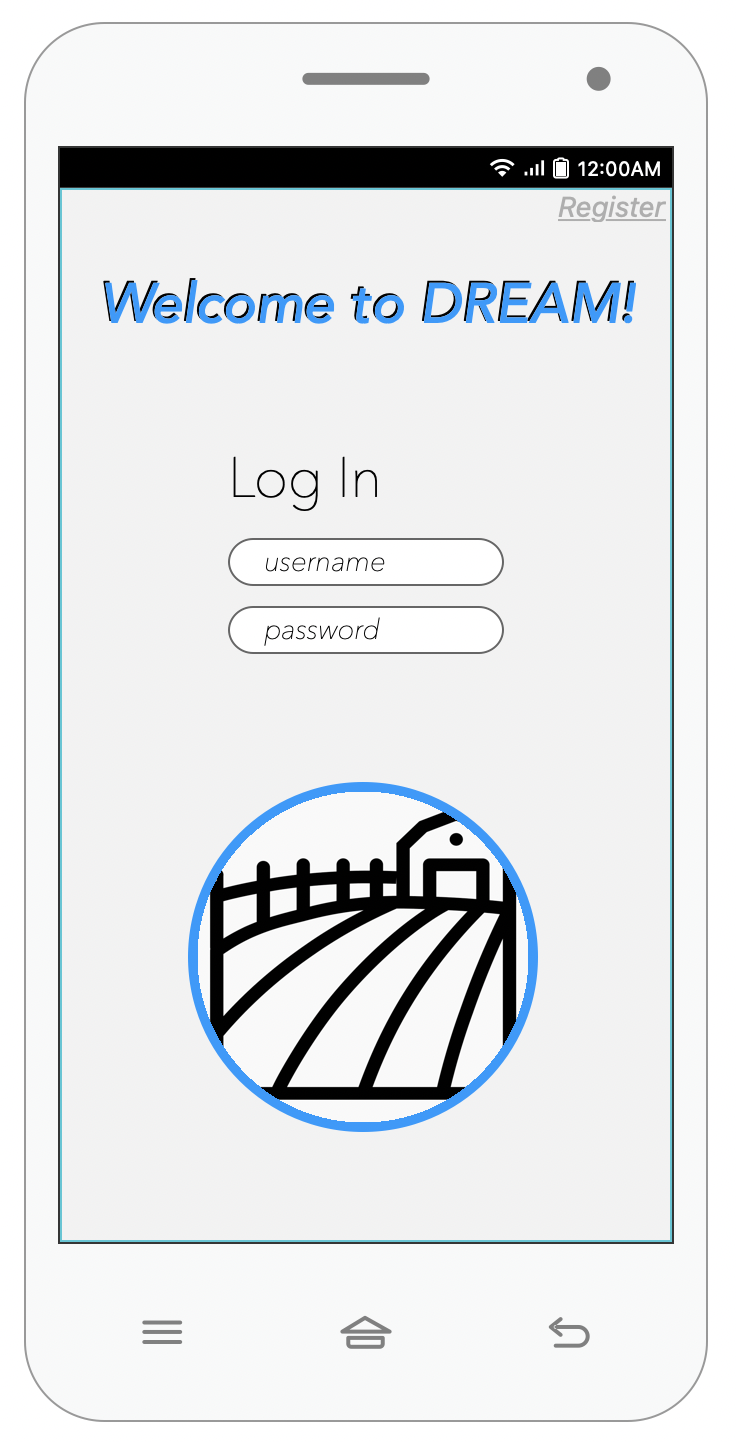
\includegraphics[scale=0.35]{../images_diagrams/mock_ups/login100.png}
\caption{\label{fig:mock_login}Login.}
\end{figure}

\begin{figure}[H]
\centering
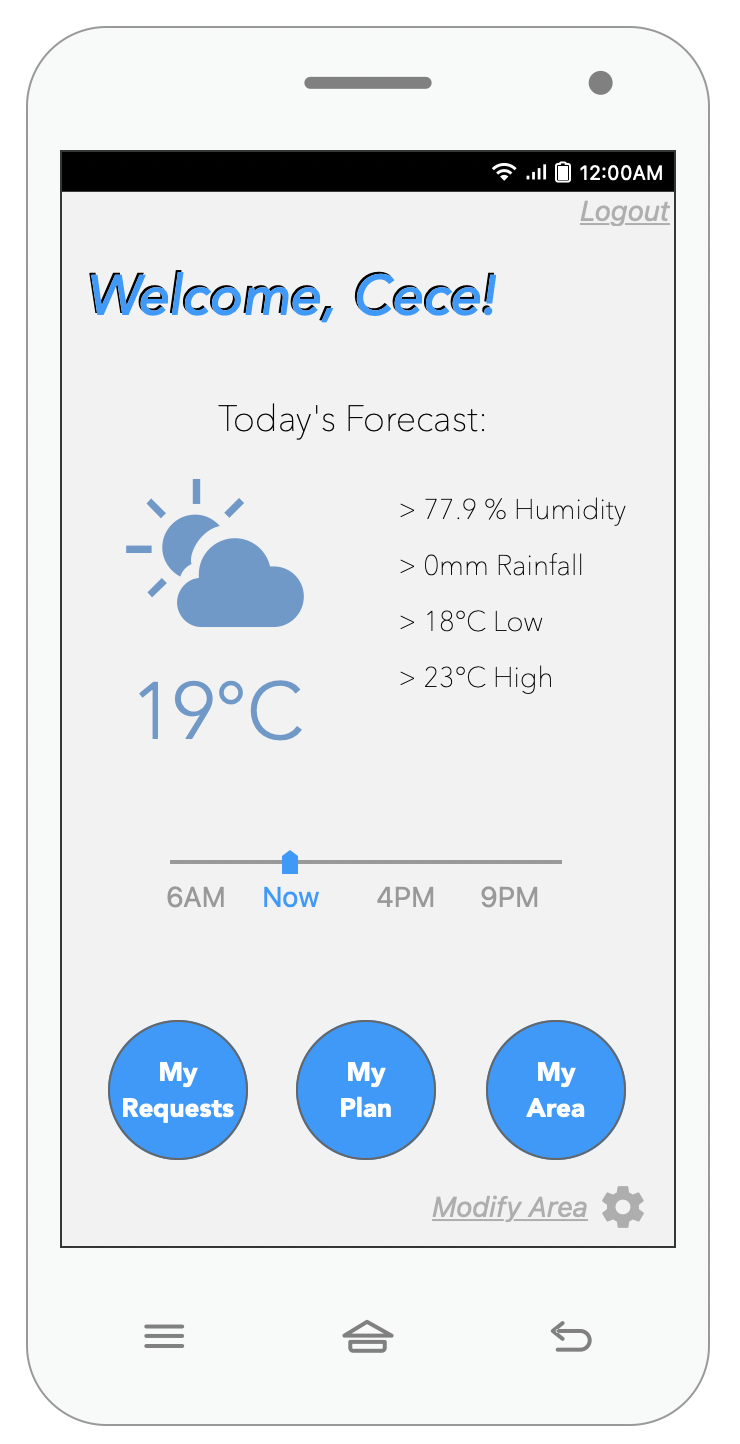
\includegraphics[scale=0.35]{../images_diagrams/mock_ups/welcomeagro100.png}
\caption{\label{fig:mock_agronomist}Agronomist home.}
\end{figure}

\begin{figure}[H]
\centering
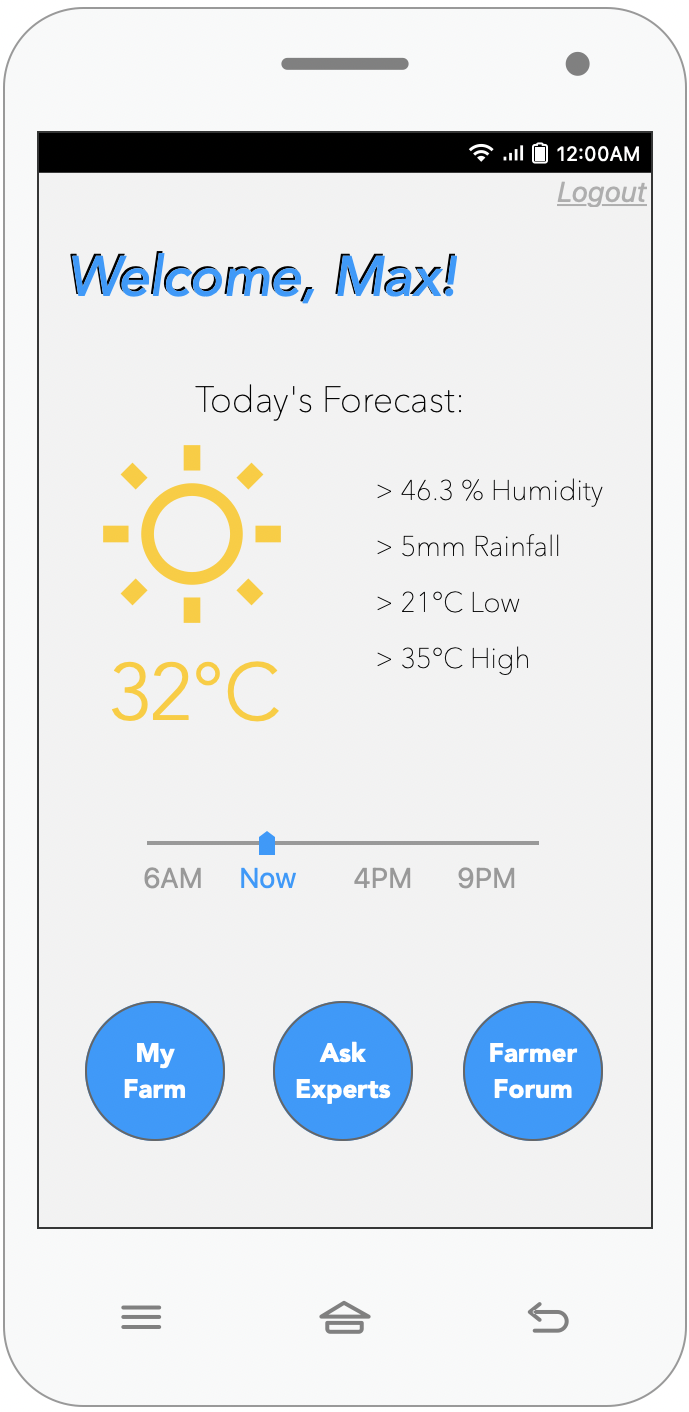
\includegraphics[scale=0.35]{../images_diagrams/mock_ups/welcomefarmer100.png}
\caption{\label{fig:mock_farmer}Farmer home.}
\end{figure}
\end{multicols}

\newpage
\subsection{Farmer Views}
\noindent
The following mock ups show some of the main interfaces for a farmer user. From a farmer's homepage as shown in Figure \ref{fig:mock_farmer}, the farmer user can either navigate to the My Farm interface, Farmer Forum interface, or the Ask Experts interface using the three blue buttons at the bottom of the screen. Figures \ref{fig:mock_farm} and \ref{fig:mock_forum} show the My Farm and the Farmer Forum pages, respectively. 

\begin{multicols}{2}
\begin{figure}[H]
\centering
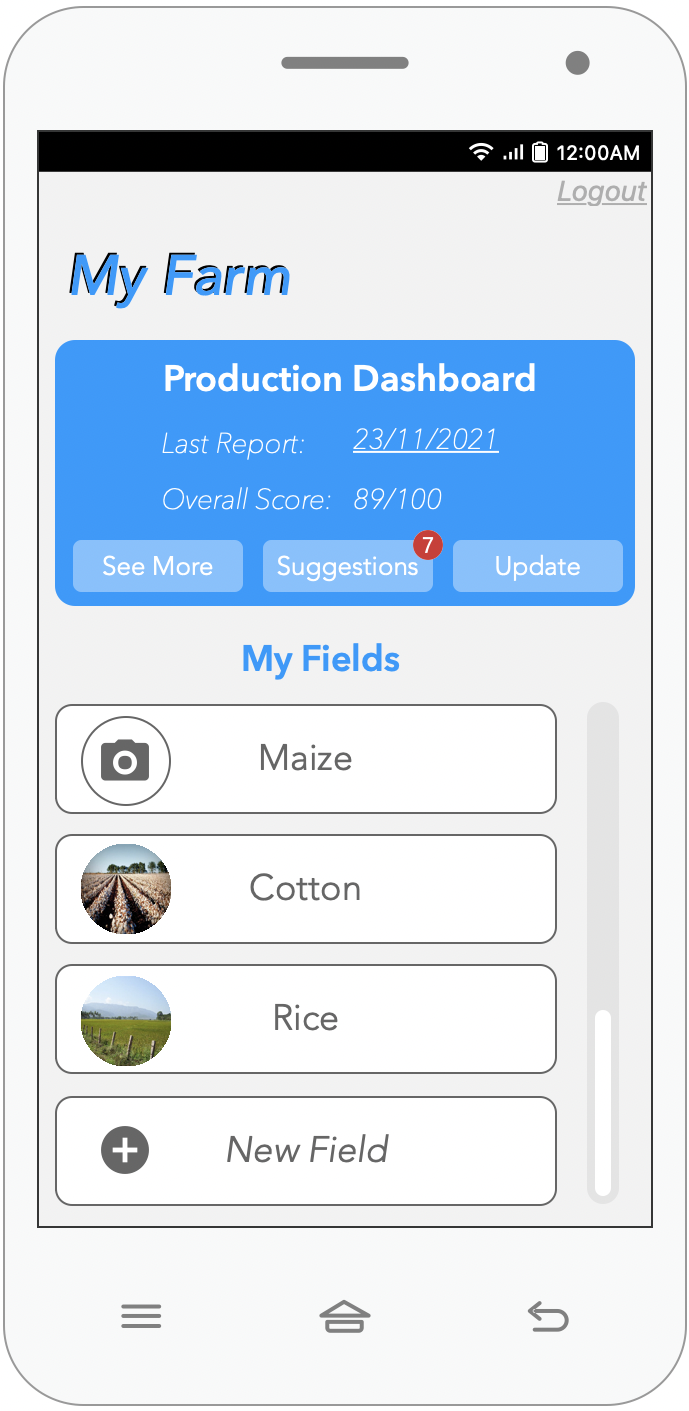
\includegraphics[scale=0.5]{../images_diagrams/mock_ups/myfarm100.png}
\caption{\label{fig:mock_farm}My Farm mock up.}
\end{figure}

\begin{figure}[H]
\centering
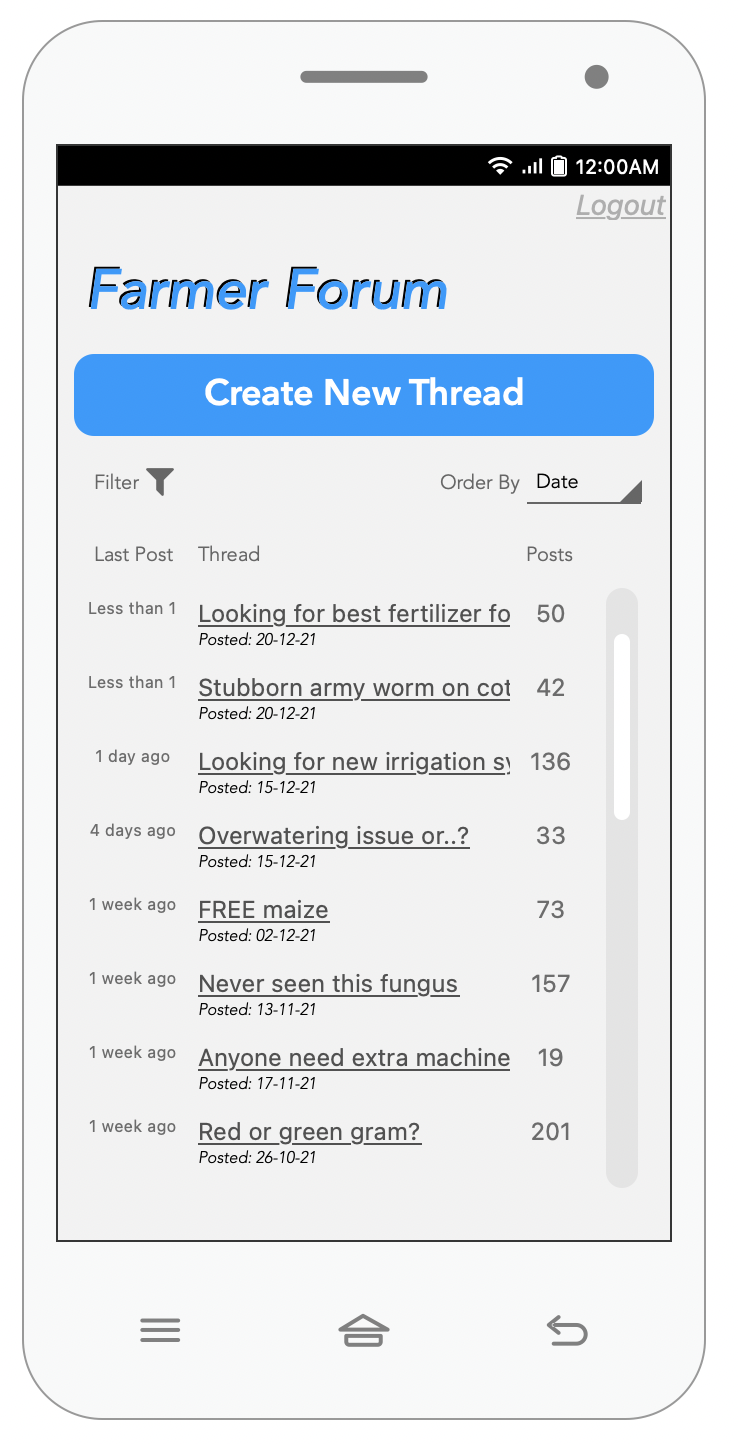
\includegraphics[scale=0.5]{../images_diagrams/mock_ups/farmerforum100.png}
\caption{\label{fig:mock_forum}Farmer Forum mock up.}
\end{figure}
\end{multicols}
\newpage 
\subsection{Farmer Request for Help}
\noindent
In order to issue a new request for help, a farmer can click on the “Ask Experts" button as shown in the bottom of Figure \ref{fig:mock_farmer}. This will navigate the user to their main inbox as shown in Figure \ref{fig:mock_inbox}. The user can see their requests as messages to their agronomist. New responses from their agronomist are highlighted and shown at the top of the list of their other messages or help requests. To issue a new help request, the farmer user can click on the “New Request" button from Figure \ref{fig:mock_inbox}. The help request form is shown in Figure \ref{fig:mock_request}.

\begin{multicols}{2}
\begin{figure}[H]
\centering
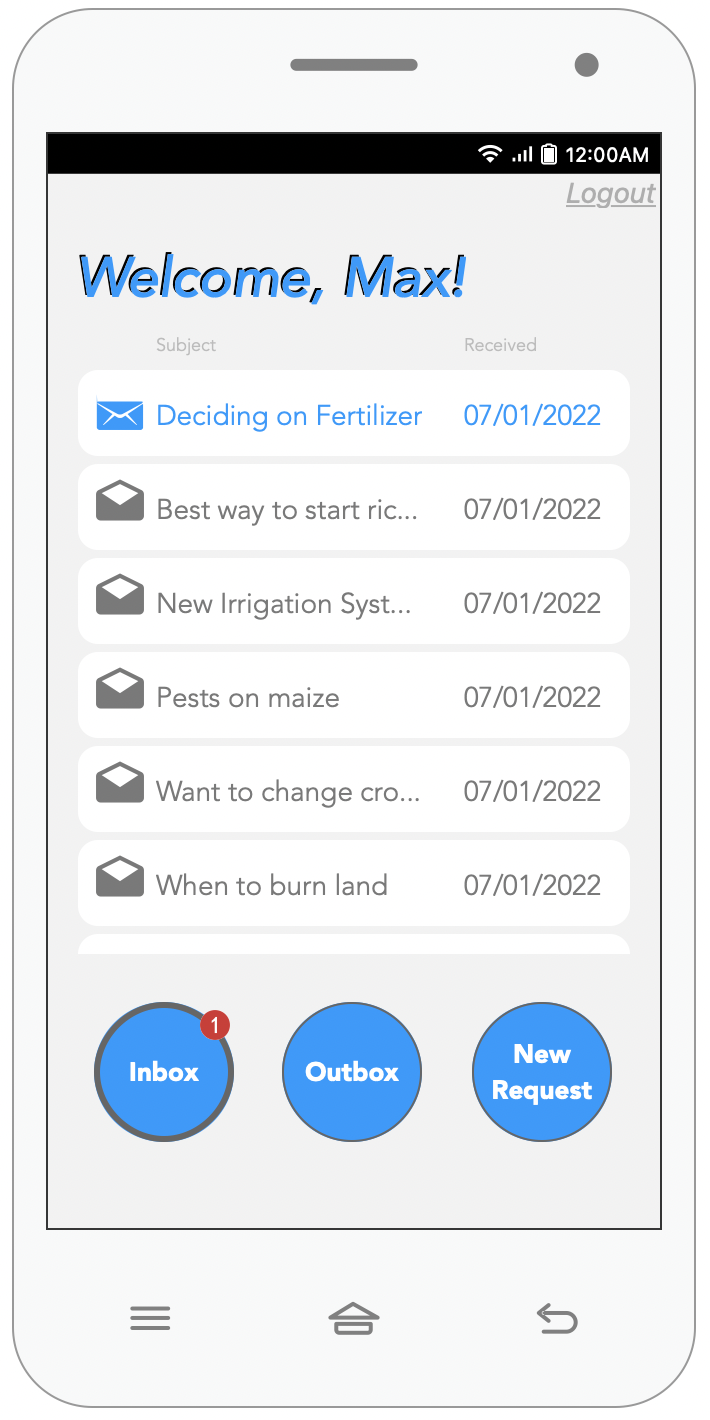
\includegraphics[scale=0.5]{../images_diagrams/mock_ups/dd/Req01_Inbox.png}
\caption{\label{fig:mock_inbox}Farmer message inbox.}
\end{figure}

\begin{figure}[H]
\centering
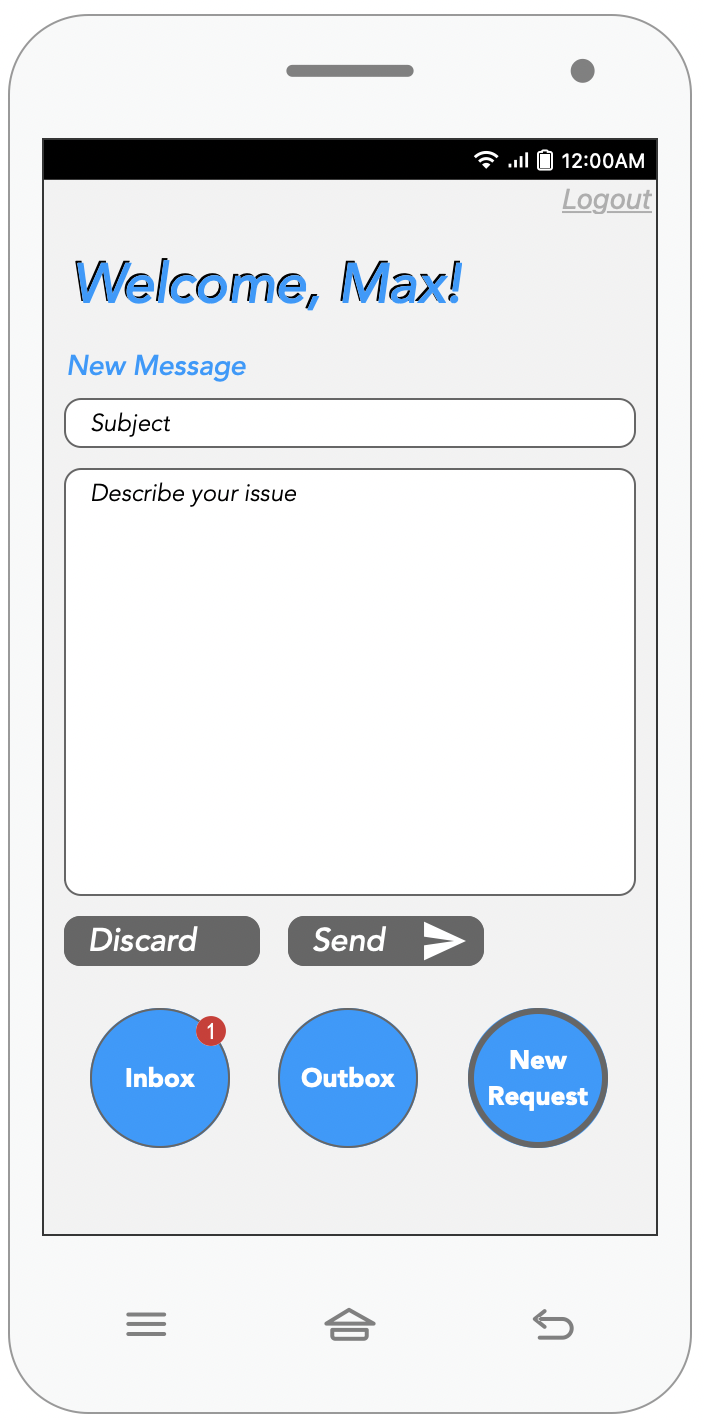
\includegraphics[scale=0.5]{../images_diagrams/mock_ups/dd/Req02_NewReq.png}
\caption{\label{fig:mock_request}Farmer new help request.}
\end{figure}
\end{multicols}

\newpage
\subsection{Agronomist Views}
\noindent
The following mock ups show some of the main interfaces for an agronomist user. From an agronomist's homepage as shown in Figure \ref{fig:mock_agronomist}, the agronomist user can either navigate to the My Requests interface, My Plan interface, or the My Area interface using the three blue buttons at the bottom of the screen. Figures \ref{fig:mock_area} and \ref{fig:mock_plan} show the My Area and the My Plan pages, respectively. The My Requests interface is very similar to that of the farmers' Help Request interface as shown in Figure \ref{fig:mock_inbox}.

\begin{multicols}{2}
 
\begin{figure}[H]
 \centering
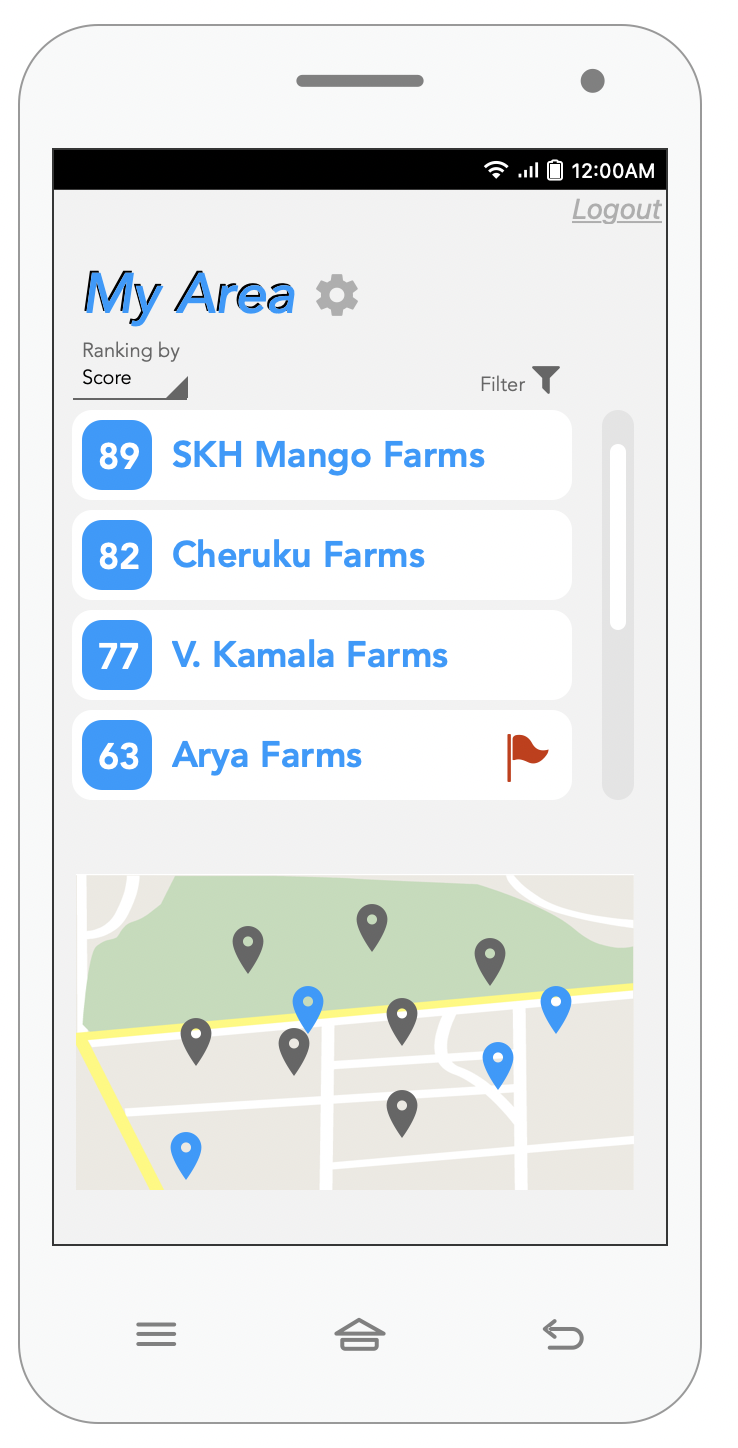
\includegraphics[scale=0.5]{../images_diagrams/mock_ups/myarea100.png}
\caption{\label{fig:mock_area}My Area agronomist mock up.}
 \end{figure}

\begin{figure}[H]
\centering
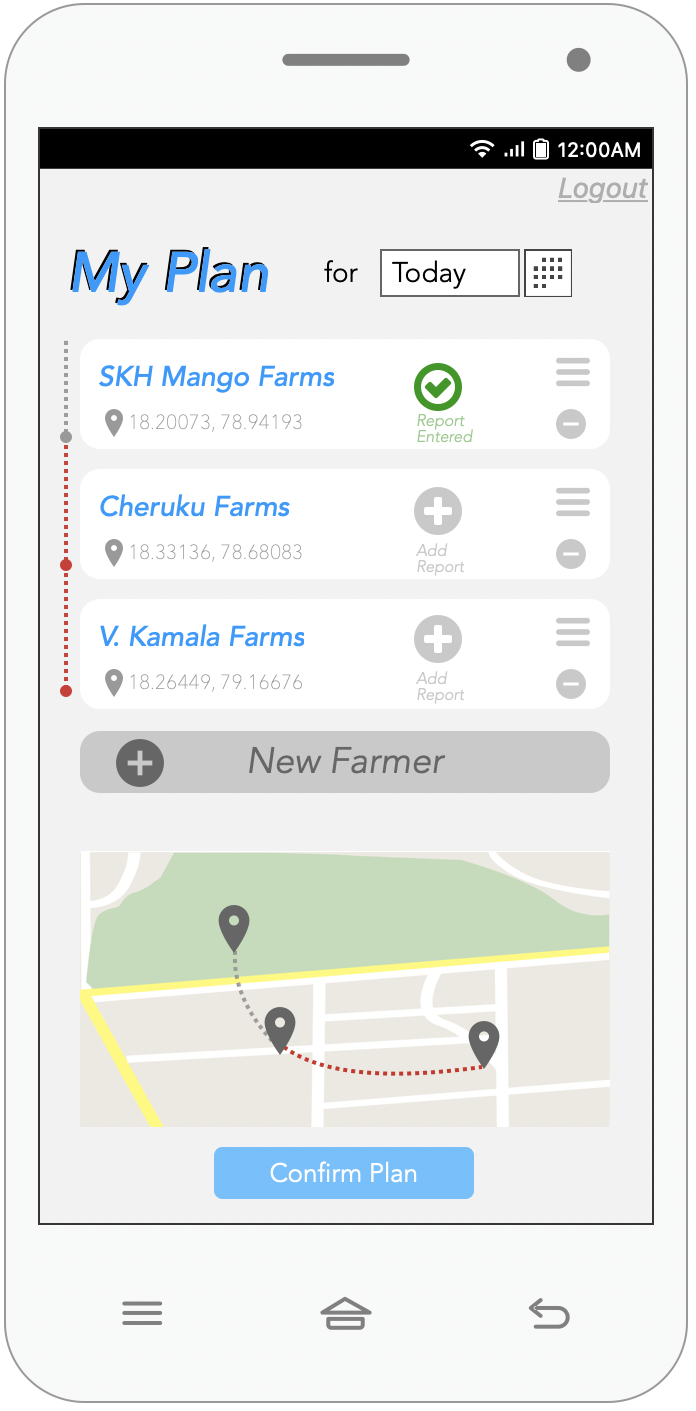
\includegraphics[scale=0.5]{../images_diagrams/mock_ups/myplan100.png}
\caption{\label{fig:mock_plan}My Plan agronomist mock up.}
\end{figure}
\end{multicols}

\newpage
\subsection{Agronomist Managing Daily Plan}
\noindent
When an agronomist user navigates to their My Plan interface using the blue button labeled “My Plan" from their homepage shown in Figure \ref{fig:mock_agronomist}, the user is navigated to a page that looks like Figure \ref{fig:mockplan_start}. The farmers listed have been automatically chosen based on the DREAM algorithm that queues farmers based on different factors such as ranking, date of last visit, help requests, and more. The user can use the three-bars button on the left-hand side of the farmers' names in order to modify the order in which the farmer's are scheduled. When the order is modified as in Figure \ref{fig:mockplan_reorder}, the map with the tentative itinerary view is also updated. 

\begin{multicols}{2}
\begin{figure}[H]
\centering
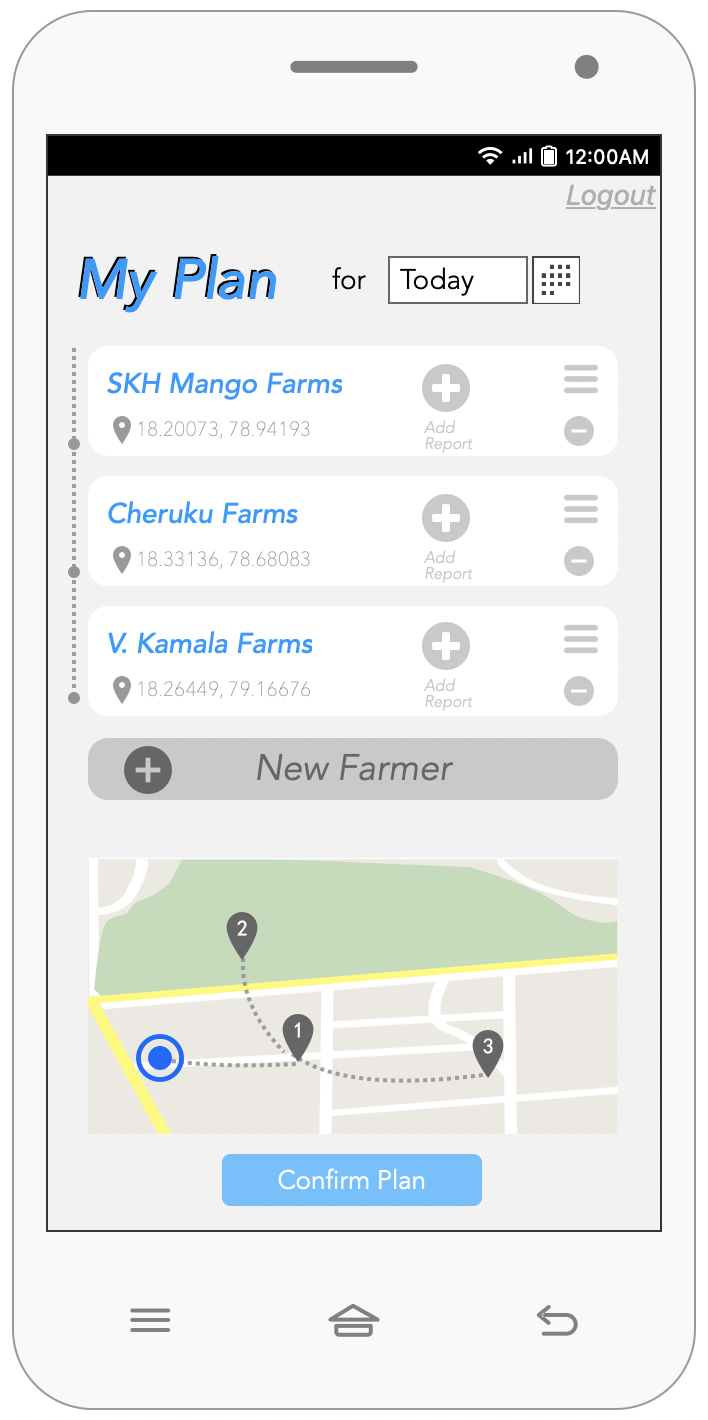
\includegraphics[scale=0.5]{../images_diagrams/mock_ups/dd/Plan01_Start.png}
\caption{\label{fig:mockplan_start}Starting a new plan}
\end{figure}

\begin{figure}[H]
\centering
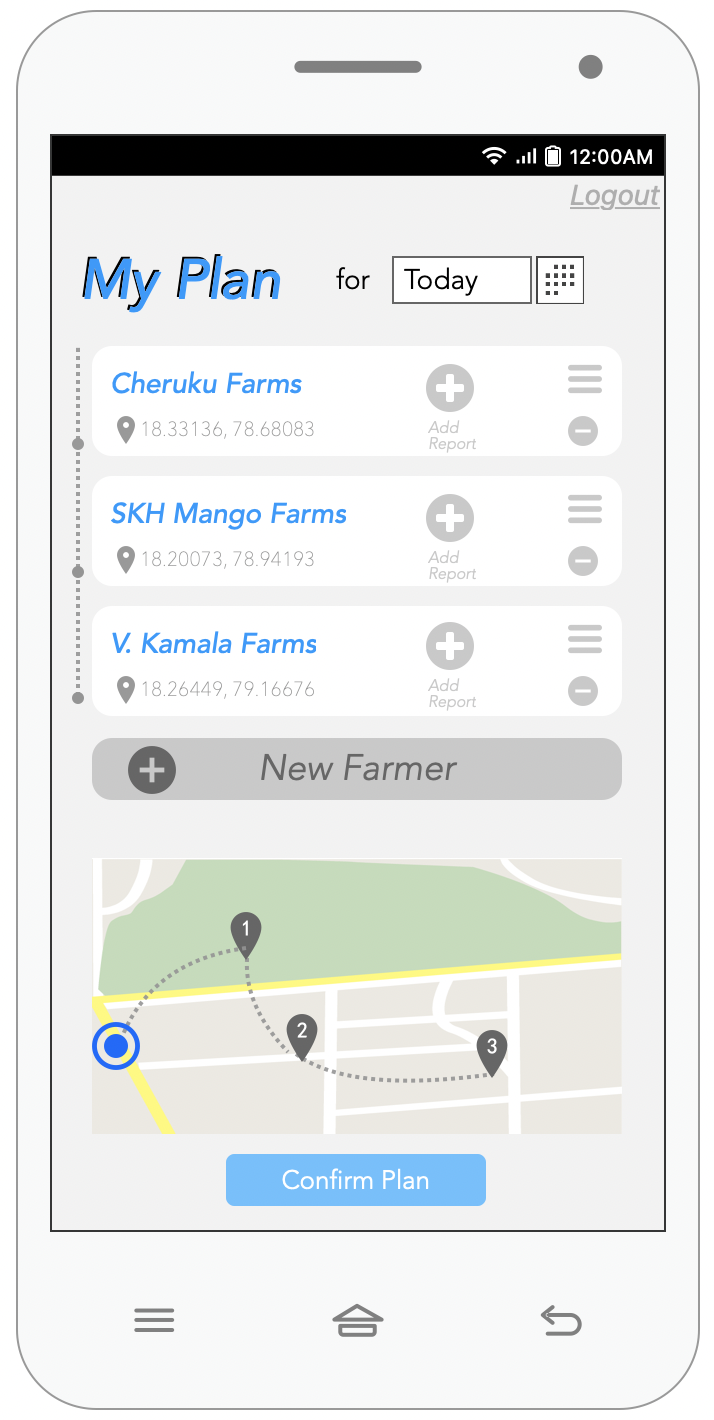
\includegraphics[scale=0.5]{../images_diagrams/mock_ups/dd/Plan02_ChangeOrder.png}
\caption{\label{fig:mockplan_reorder}Modify order of visits.}
\end{figure}
\end{multicols}

\newpage
\noindent
When the agronomist user clicks on the address or the GPS coordinates below the corresponding farm name, the user is prompted to start the navigation guidance as shown in Figure \ref{fig:mockplan_nav}. If the user consented to GPS tracking, the user is shown turn-by-turn navigation directions as shown in Figure \ref{fig:mockplan_guide}.

\begin{multicols}{2}
\begin{figure}[H]
\centering
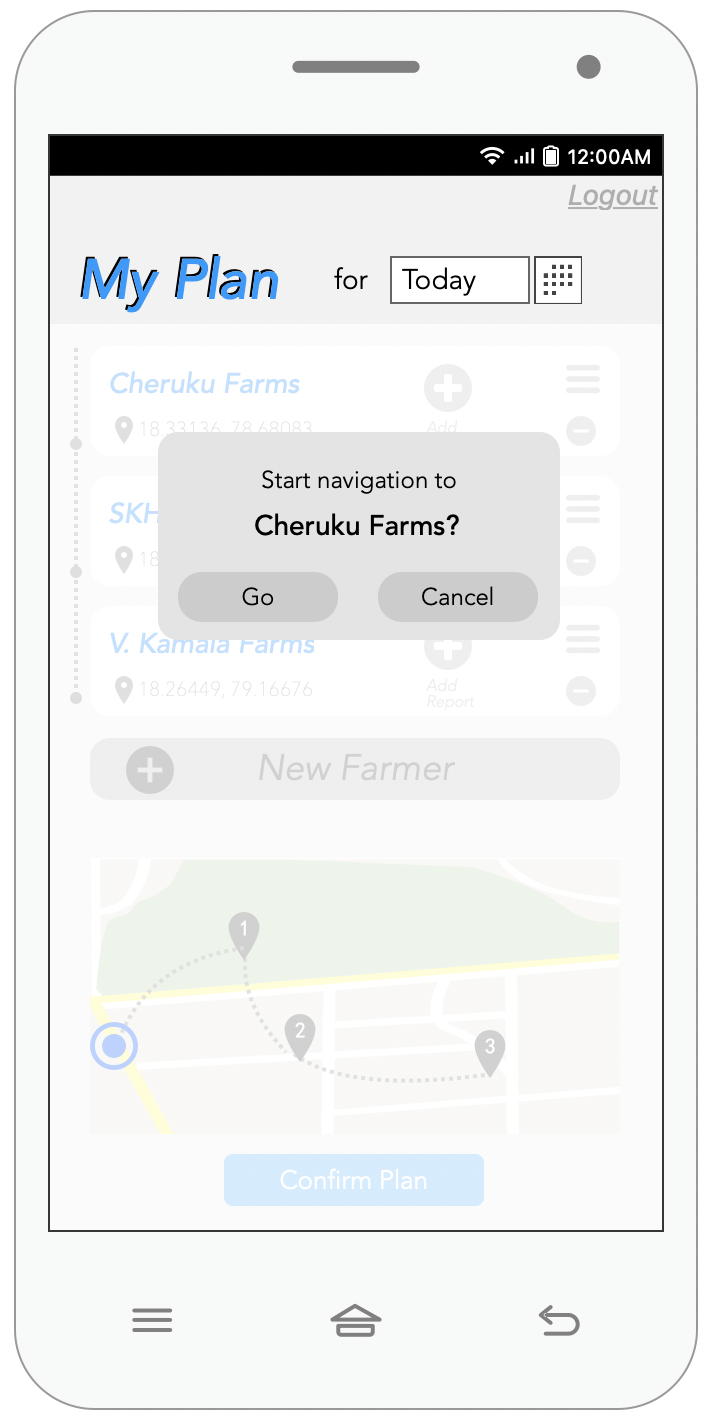
\includegraphics[scale=0.5]{../images_diagrams/mock_ups/dd/Plan03_StartNav.png}
\caption{\label{fig:mockplan_nav}Start navigation.}
\end{figure}

\begin{figure}[H]
\centering
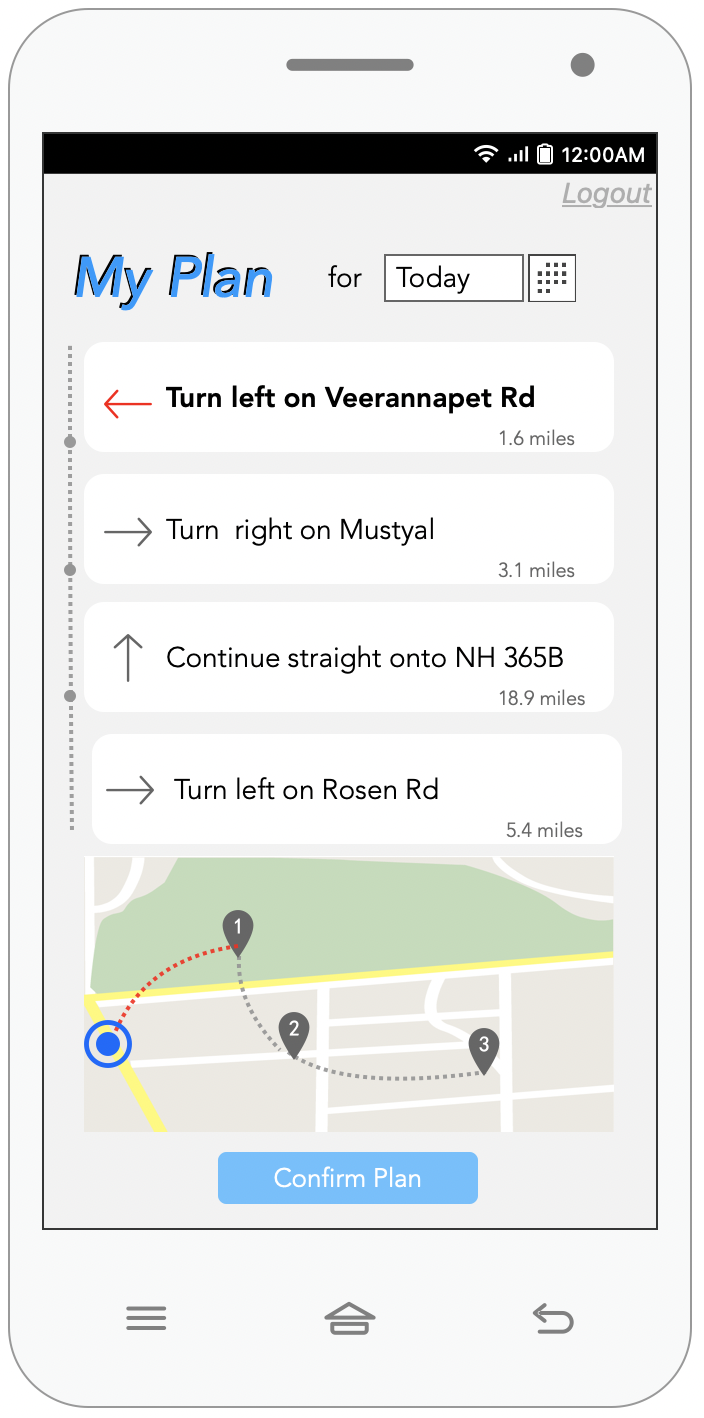
\includegraphics[scale=0.5]{../images_diagrams/mock_ups/dd/Plan04_Guidance.png}
\caption{\label{fig:mockplan_guide}Navigation guidance.}
\end{figure}
\end{multicols}

\newpage
\noindent
After the agronomist has arrived to one of the farm destinations, they will see the screen on Figure \ref{fig:mockplan_visit}. Here, the agronomist can see the time left for the scheduled visit and choose one of three different operations: enter the report for that visit, start navigation for the next farmer, or add a new farmer to the plan. If the agronomist chooses to enter the information for the report, they will be navigated for a form as shown in Figure \ref{fig:mockplan_report}. Otherwise, if the agronomist enters a new farmer to the plan, they will return back to the plan homepage as in Figure \ref{fig:mockplan_start}. Again, the agronomist can reorder and modify the plan as they wish but the agronomist is responsible for entering the data for the reports, so it is helpful to complete the report forms directly during the farm visits.


\begin{multicols}{2}
\begin{figure}[H]
\centering
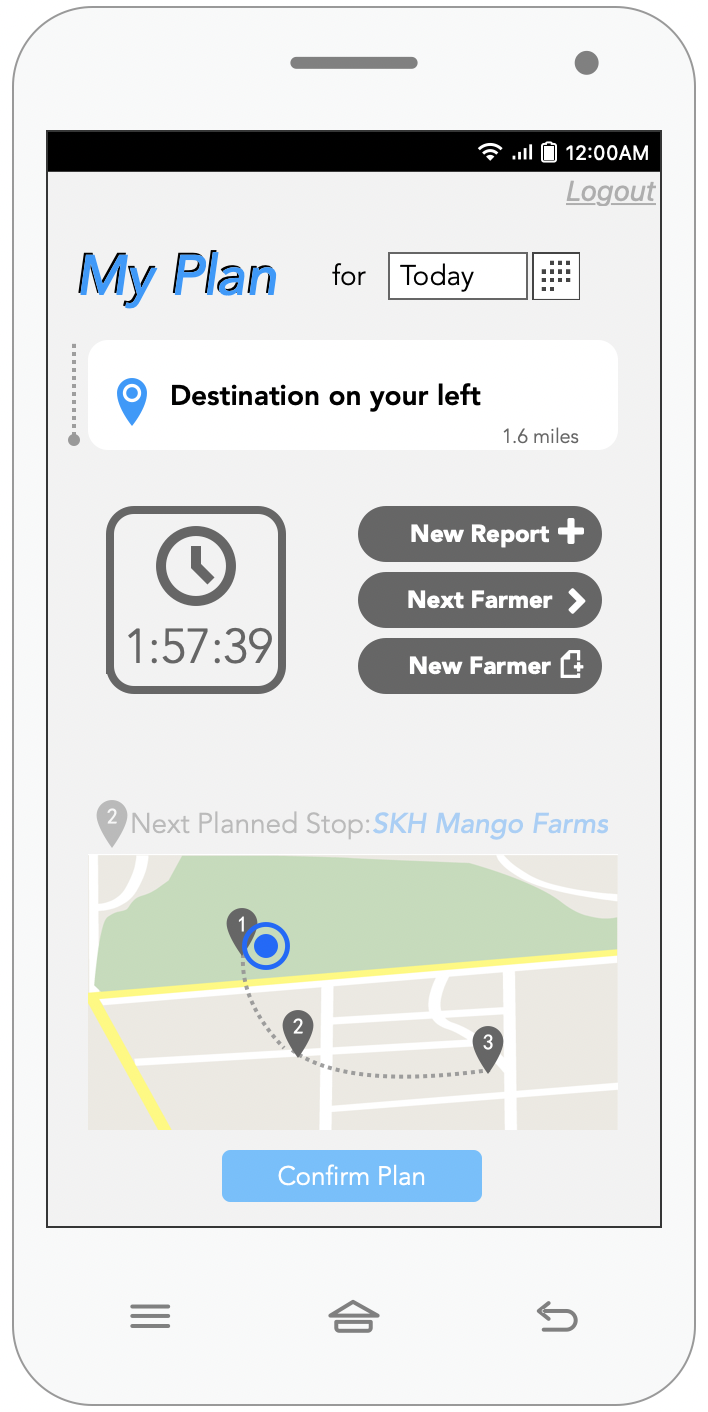
\includegraphics[scale=0.5]{../images_diagrams/mock_ups/dd/Plan05_AtFarm.png}
\caption{\label{fig:mockplan_visit}During a visit.}
\end{figure}

\begin{figure}[H]
\centering
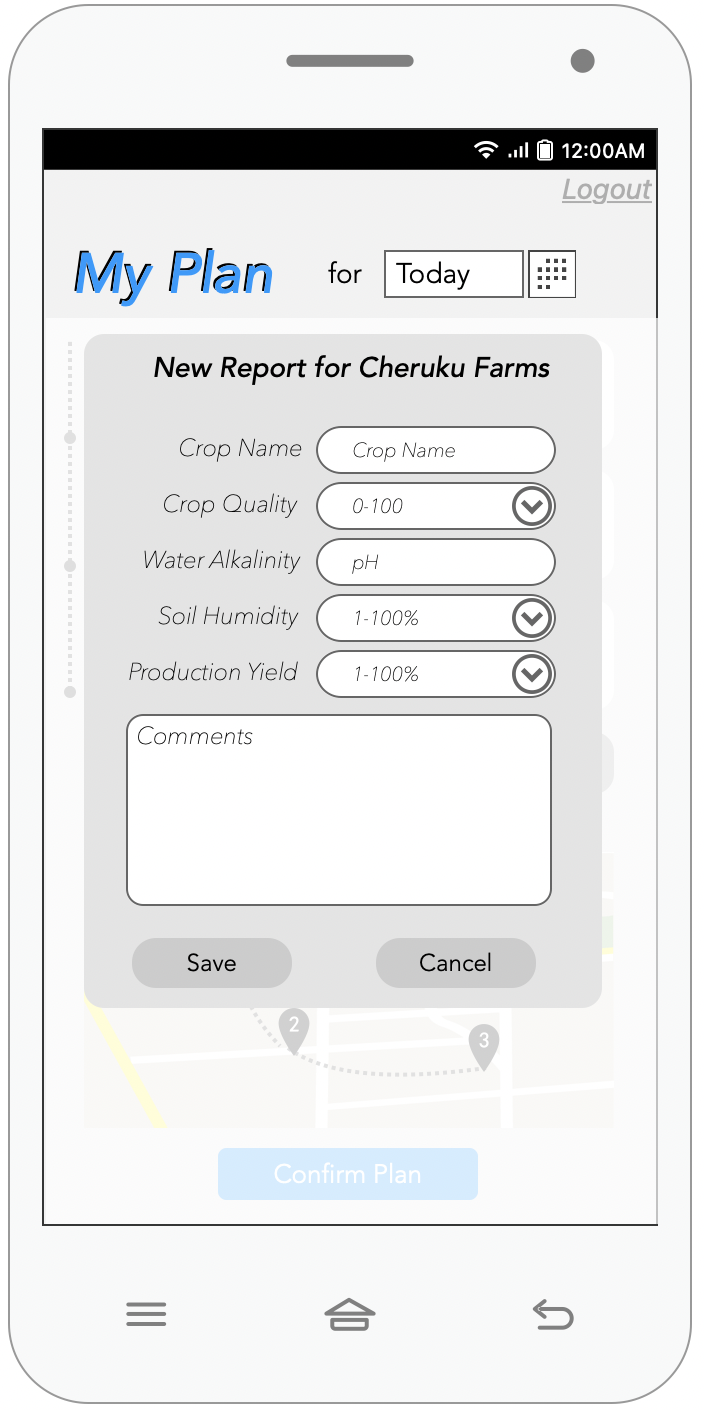
\includegraphics[scale=0.5]{../images_diagrams/mock_ups/dd/Plan06_NewReport.png}
\caption{\label{fig:mockplan_report}New report form.}
\end{figure}
\end{multicols}

\newpage
\noindent
Once the report is entered, the agronomist user is navigated back to the main My Plan homepage as shown in Figure \ref{fig:mockplan_reportentered}. Here, the interface indicates that one report has been entered. Using the application, the agronomist can continue executing their plan by going to their scheduled farm visits and entering the associated reports. After all the reports have been entered, the agronomist will see a screen as shown in Figure \ref{fig:mockplan_done}. Again, the agronomist is encouraged to check that all the information about the plan, including the order of the visits and the content of the reports, is accurate. When all the reports are entered, the “Confirm Plan" button becomes active as indicated by the color change. 

\begin{multicols}{2}

\begin{figure}[H]
\centering
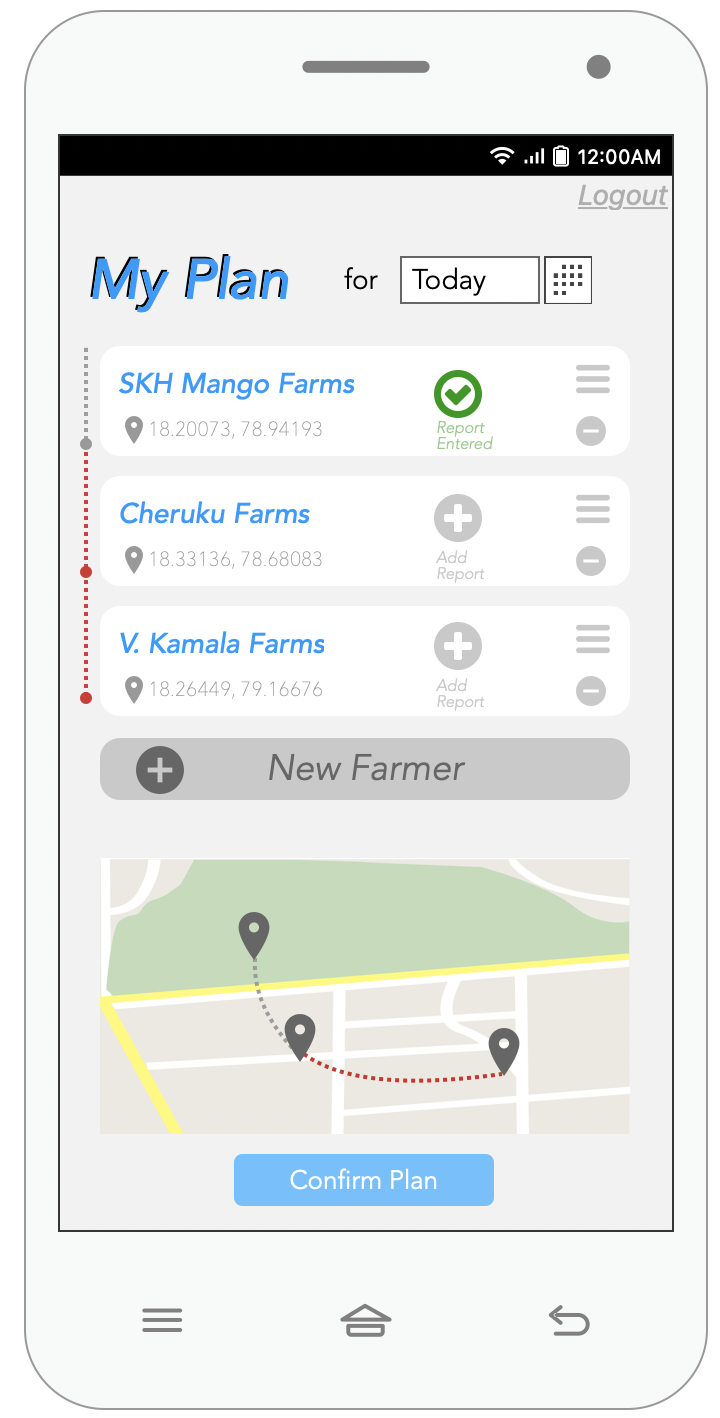
\includegraphics[scale=0.5]{../images_diagrams/mock_ups/dd/Plan07_OneReport.png}
\caption{\label{fig:mockplan_reportentered}First report entered.}
\end{figure}

\begin{figure}[H]
\centering
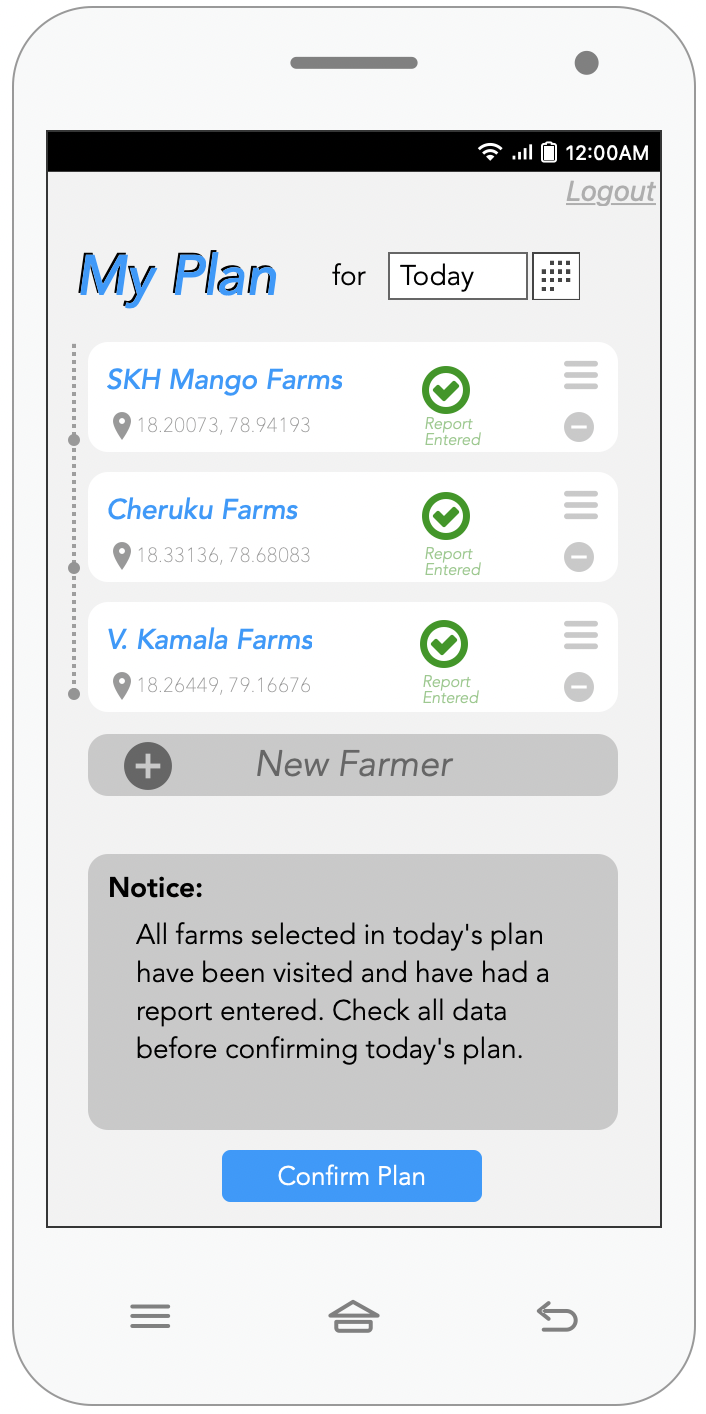
\includegraphics[scale=0.5]{../images_diagrams/mock_ups/dd/Plan08_AllReportsEntered.png}
\caption{\label{fig:mockplan_done}All reports entered.}
\end{figure}

\end{multicols}


\newpage
\subsection{Policy Maker View}
\noindent
When the policy maker user logs in with valid credentials, they are navigated to their homepage view as shown in Figure \ref{fig:mockpolicy_dash}. Policy makers can see a summary of the data in the top left-hand tile, filter their ranking on the bottom left-hand tile, see the farmers from the ranking in a map-view on the bottom right-hand tile, and access their Trigger Dashboard in the top right-hand tile. 

\begin{figure}[H]
\centering
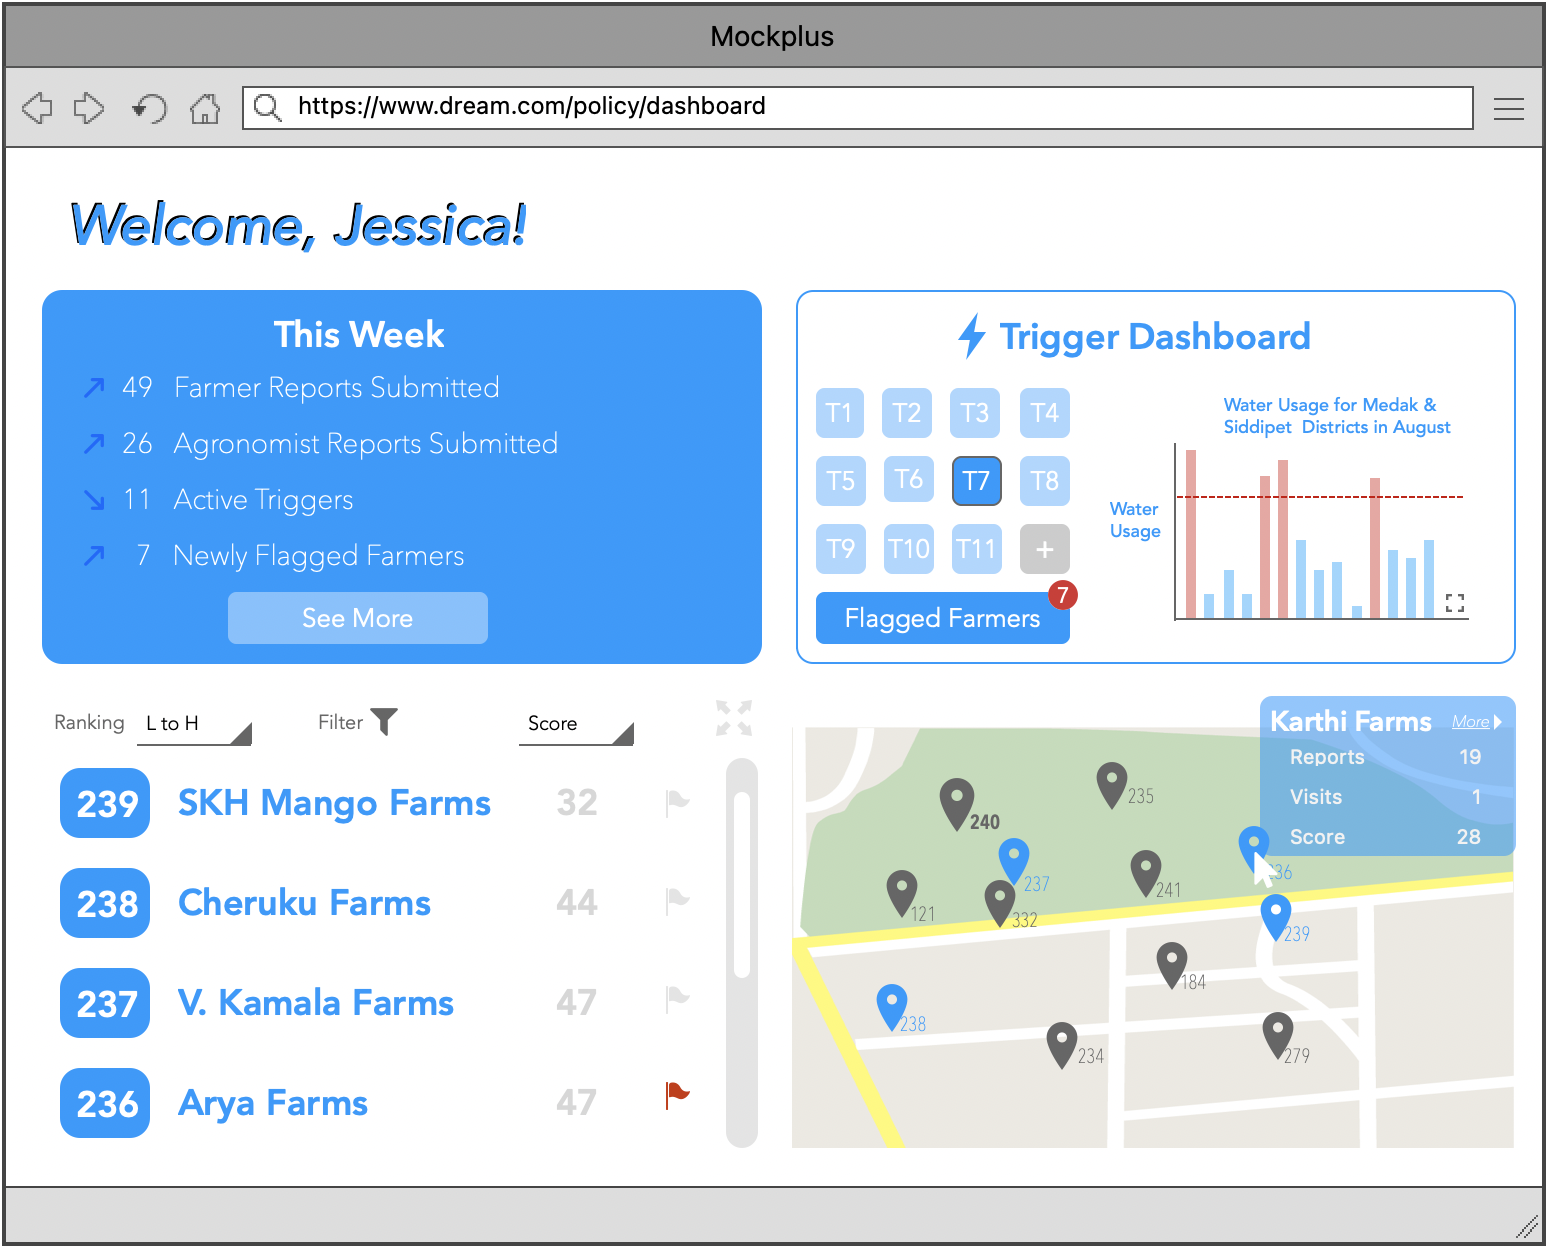
\includegraphics[scale=0.35]{../images_diagrams/mock_ups/policydash100.png}
\caption{\label{fig:mockpolicy_dash}Policy maker homepage.}
\end{figure}

\subsection{Policy Maker Setting New Trigger}
\noindent
To add a new trigger, the policy maker simply clicks on the grey plus button in the Trigger Dashboard as indicated by the cursor in Figure \ref{fig:mockpolicy_newtrig}.

\begin{figure}[H]
\centering
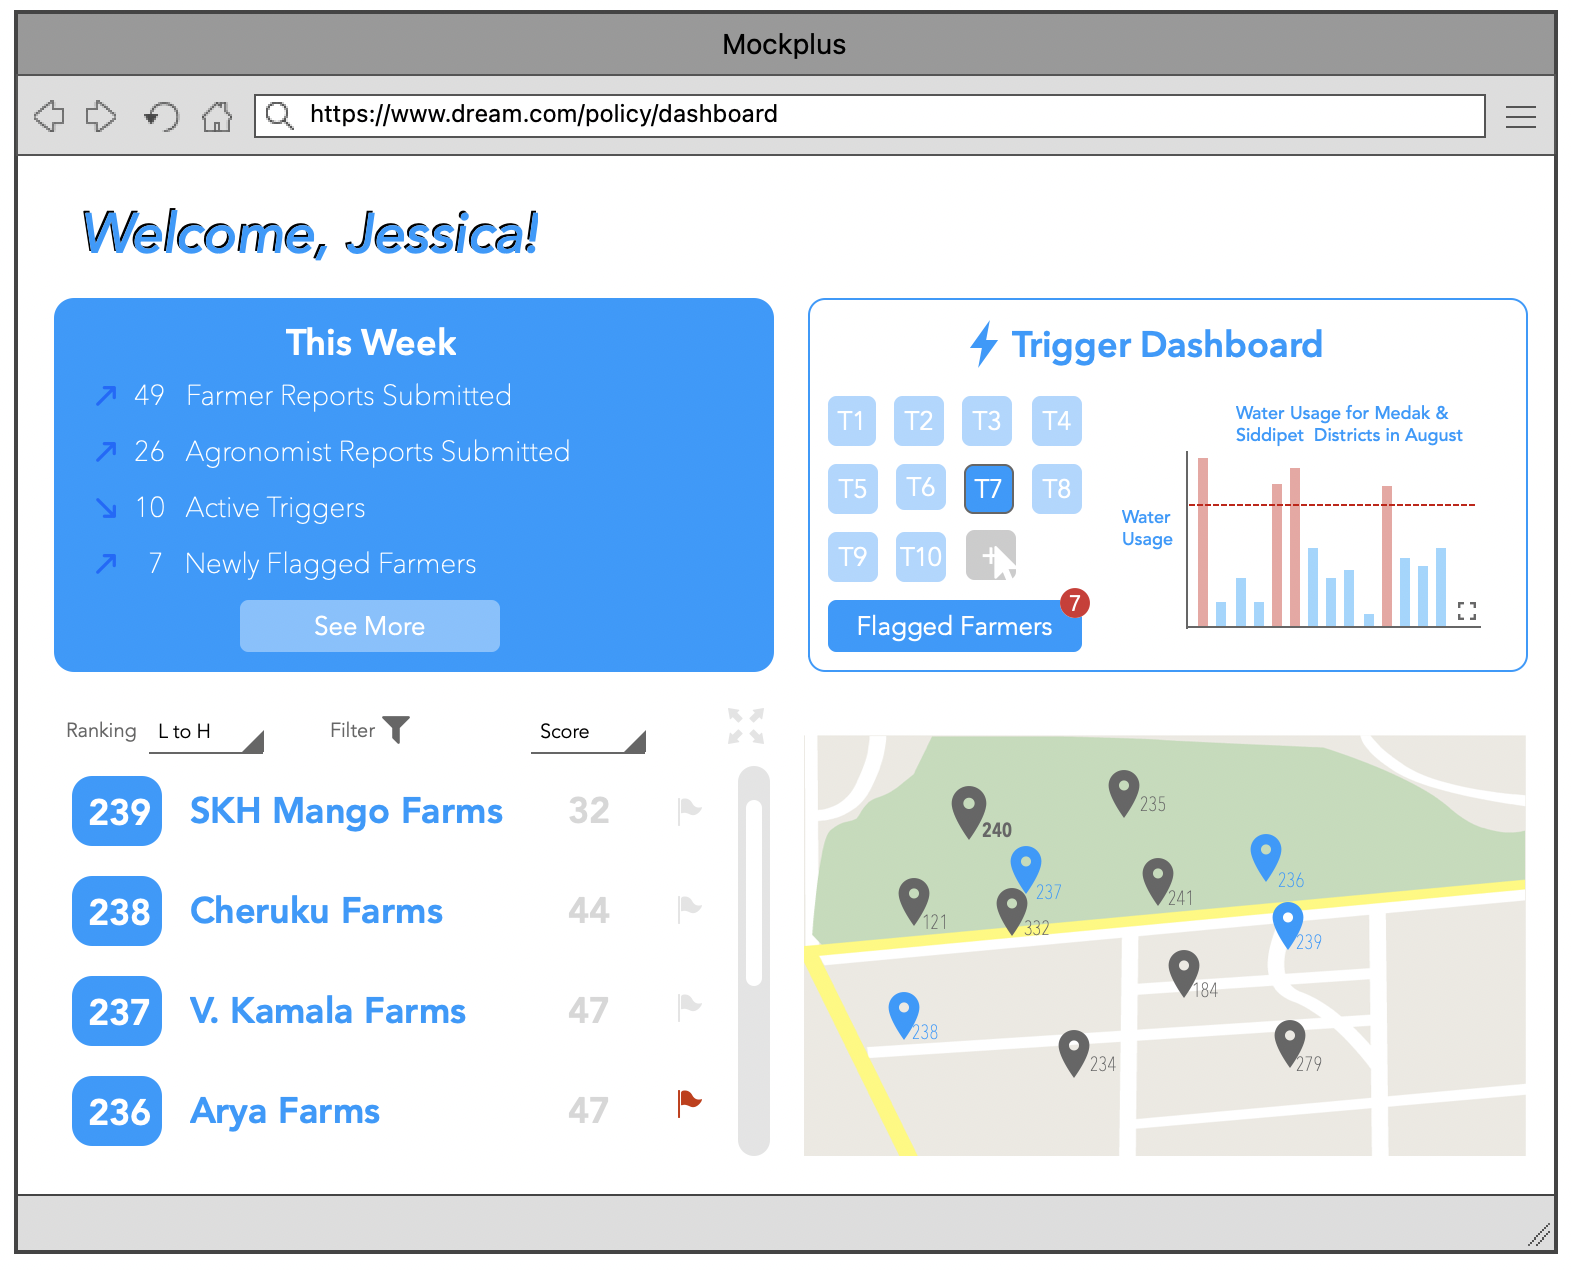
\includegraphics[scale=0.35]{../images_diagrams/mock_ups/dd/Trig01_NewTrig.png}
\caption{\label{fig:mockpolicy_newtrig}Launching new trigger form.}
\end{figure}

\noindent
The policy maker can configure a new trigger with the following options: the districts or areas to include; a specific time duration or limit to expire the trigger, optional; the crops to include in the trigger; the parameter to define the trigger over; and the maximum and minimum limits to define the trigger over. These options are also shown in Figures \ref{fig:mockpolicy_form}, \ref{fig:mockpolicy_selParam}, and \ref{fig:mockpolicy_selCrops}. 

\begin{figure}[H]
\centering
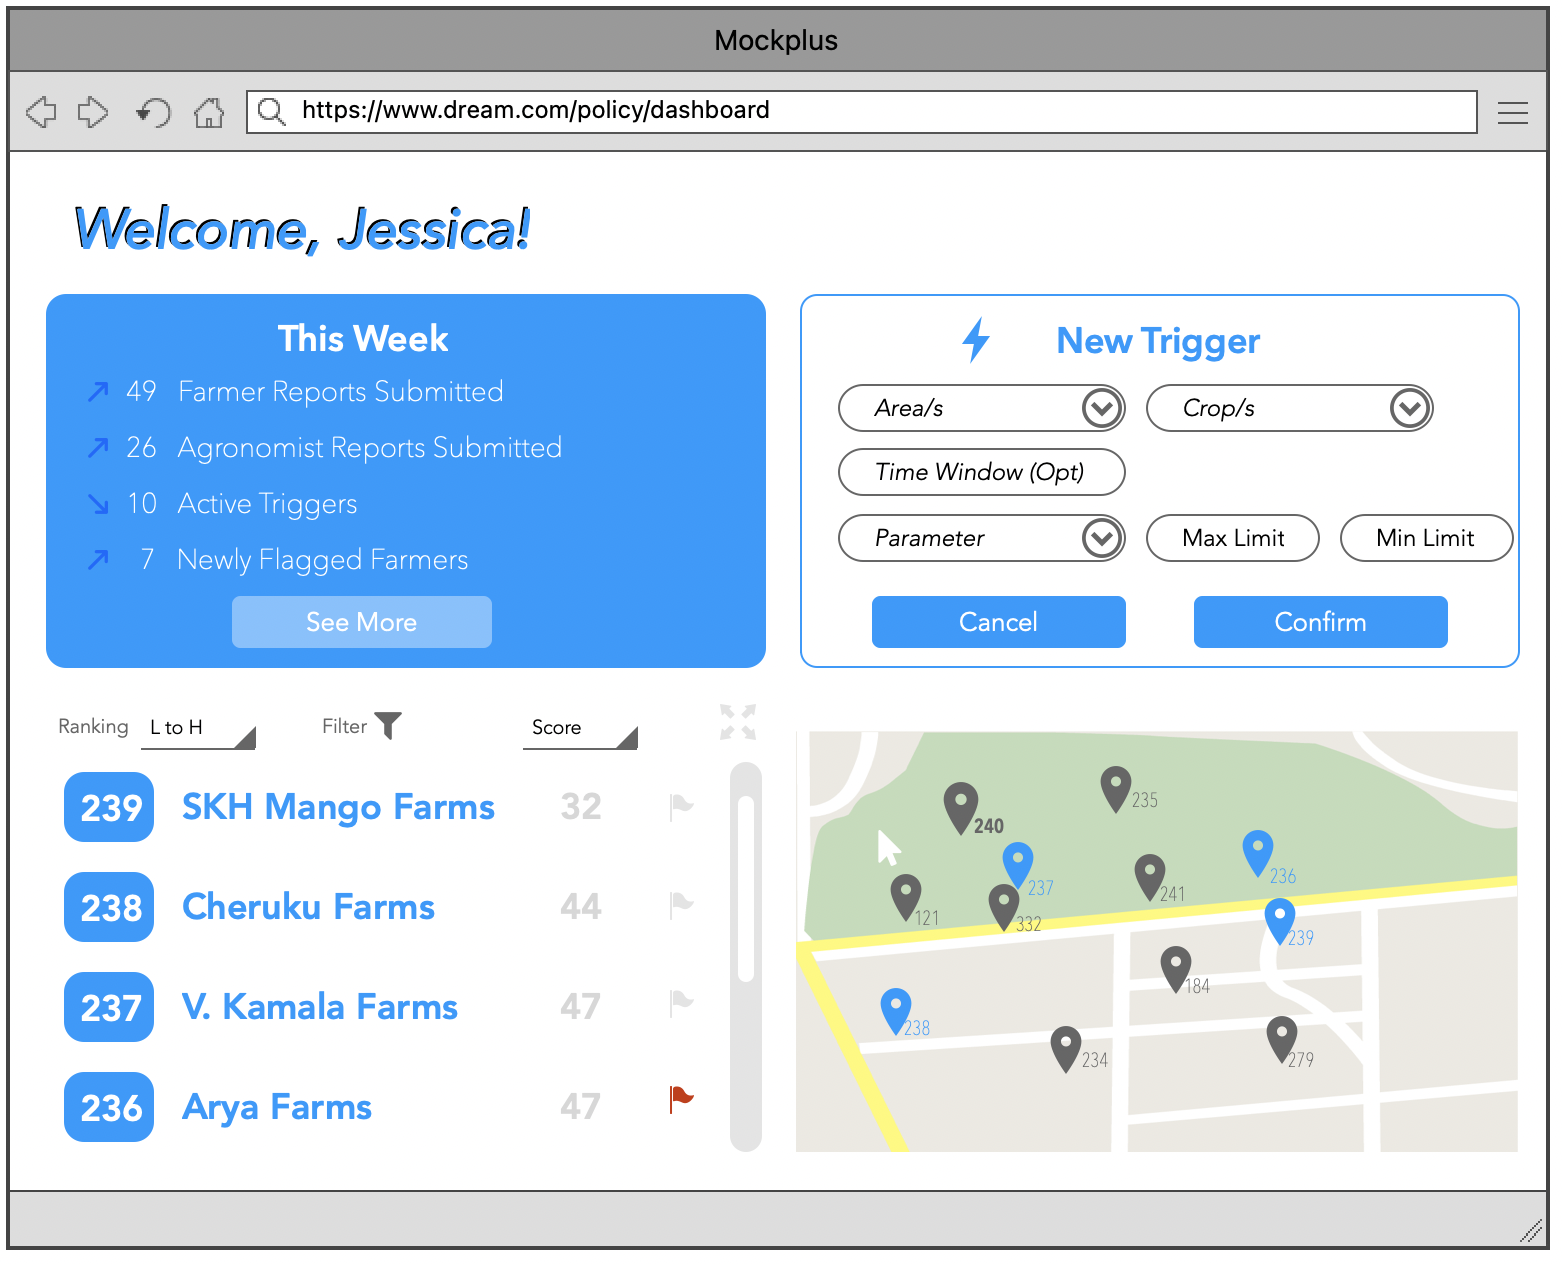
\includegraphics[scale=0.35]{../images_diagrams/mock_ups/dd/Trig02_SetUp.png}
\caption{\label{fig:mockpolicy_form}Blank new trigger form.}
\end{figure}

\noindent
As shown in Figure \ref{fig:mockpolicy_selParam}, triggers can be configured around numerical data such as overall score as determined by the DREAM algorithms, crop quality as rated by agronomists in their reports, production yield as calculated by the data provided by farmers, soil humidity as measured by the sensors deployed by TSDPS, water usage as determined by weather data compared with data provided by farmers, or water alkalinity as measured by agronomists during their farm visits. If a farm becomes associated with data that falls within the range of the minimum and maximum of the parameter defined by the trigger (and the other conditions defined by the trigger are met), the flag is set for that farmer. 


\begin{figure}[H]
\centering
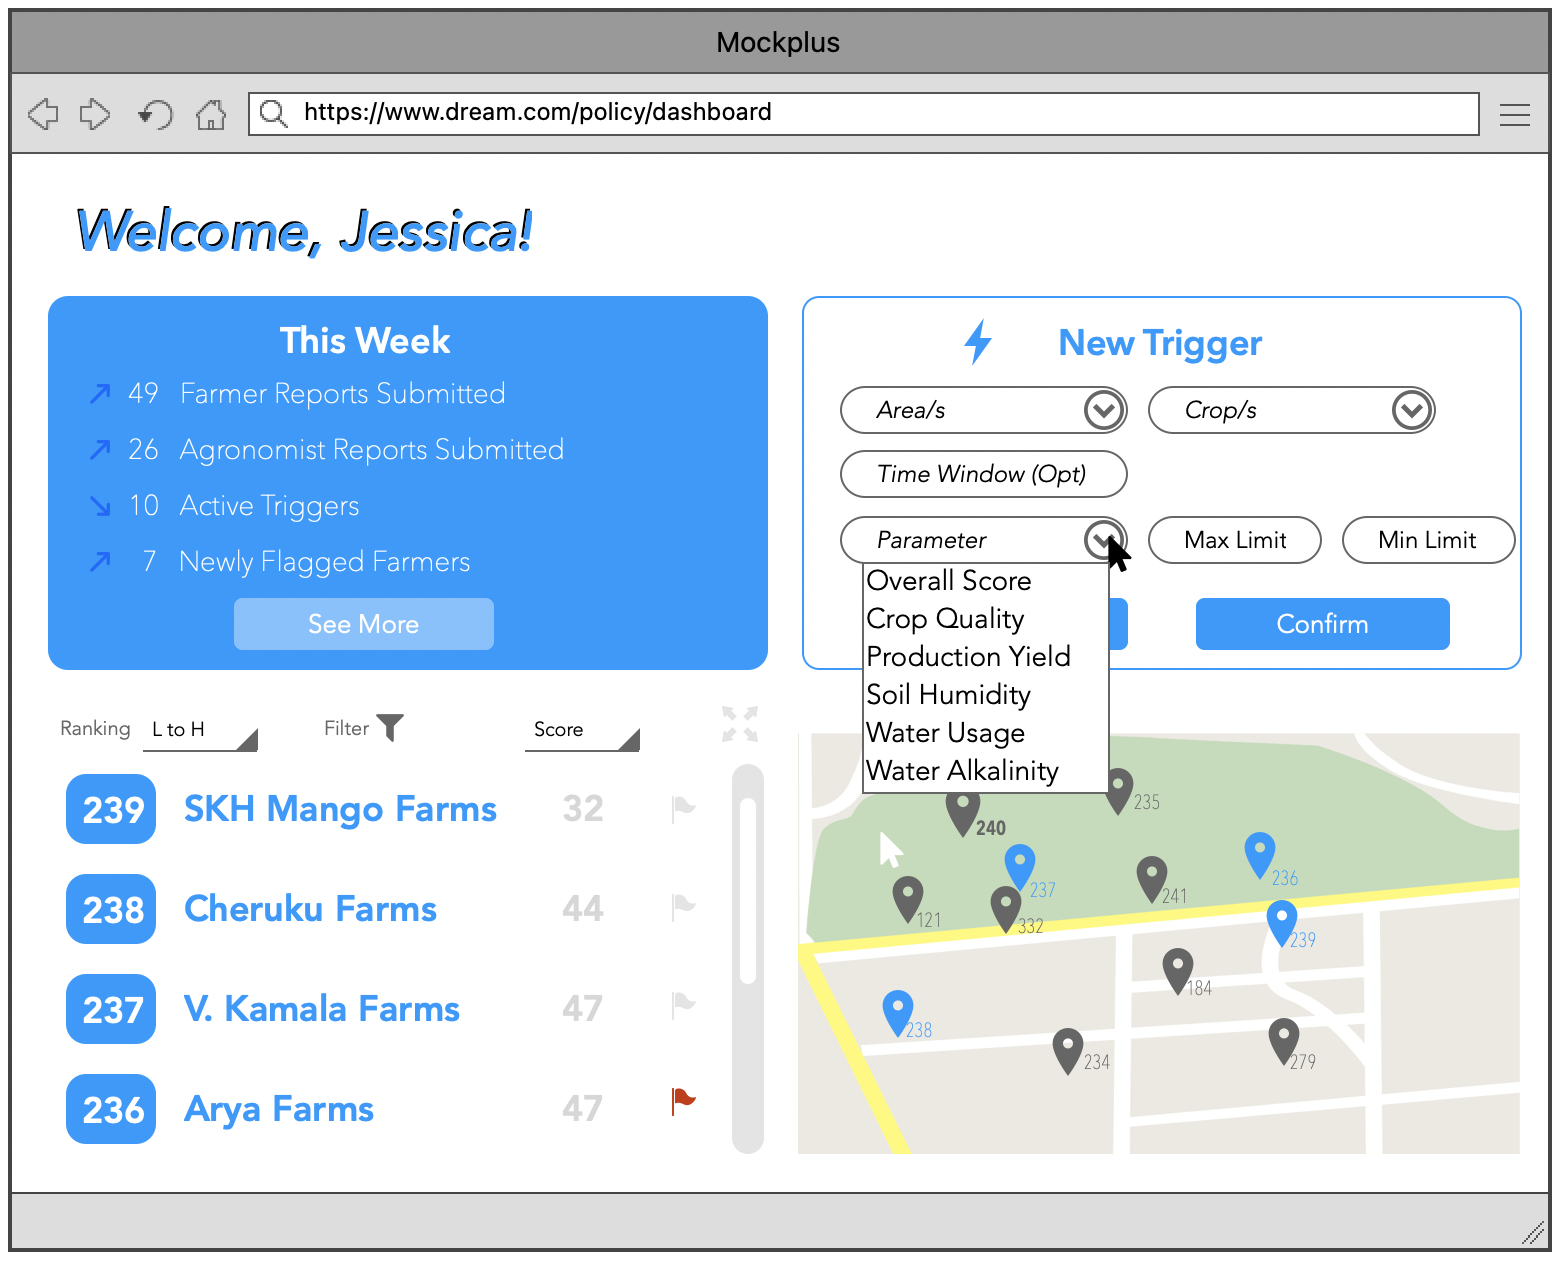
\includegraphics[scale=0.35]{../images_diagrams/mock_ups/dd/Trig03_Parameters.png}
\caption{\label{fig:mockpolicy_selParam}Select the parameter for trigger.}
\end{figure}

\noindent
As shown in Figure \ref{fig:mockpolicy_selCrops}, triggers can be set to only be relevant for farms involved in farming specific crops. Alternatively, all crops can be selected in order to ensure farmers of all crops are included in the trigger. 

\begin{figure}[H]
\centering
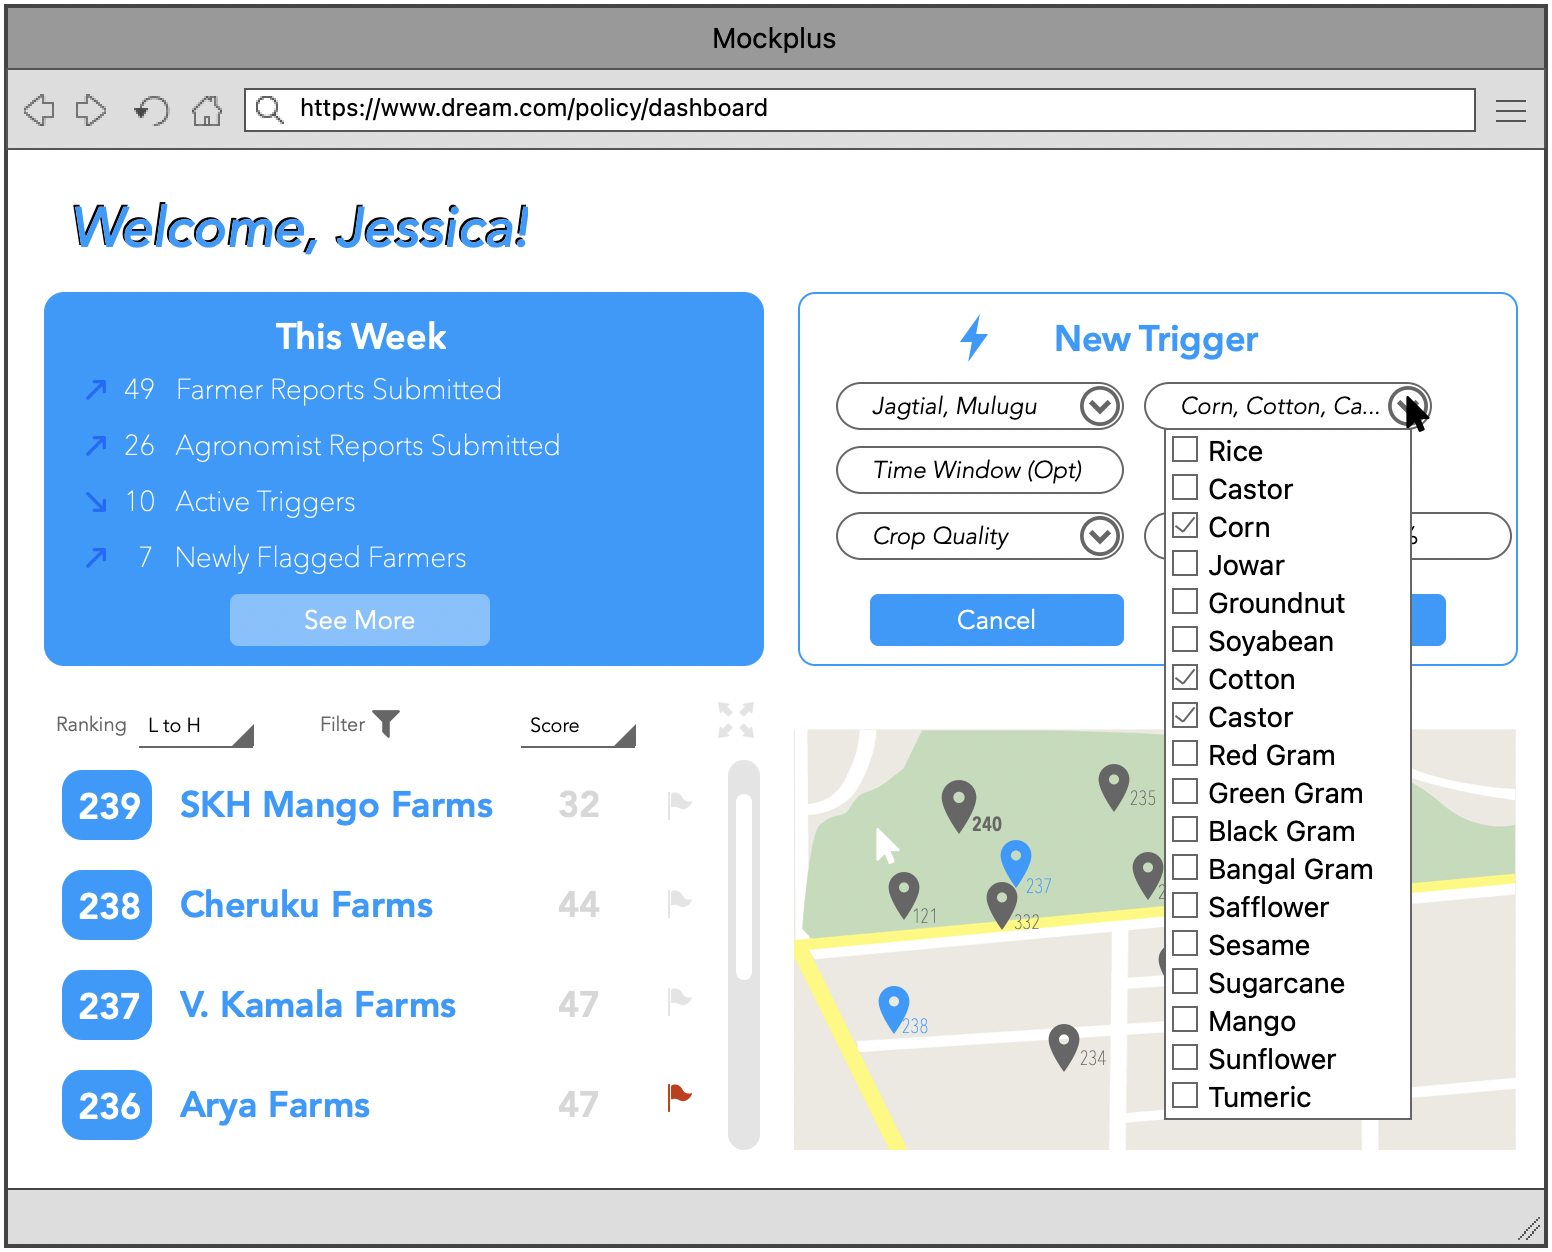
\includegraphics[scale=0.35]{../images_diagrams/mock_ups/dd/Trig04_Crops.png}
\caption{\label{fig:mockpolicy_selCrops}Select crops related to trigger.}
\end{figure}

\begin{figure}[H]
\centering
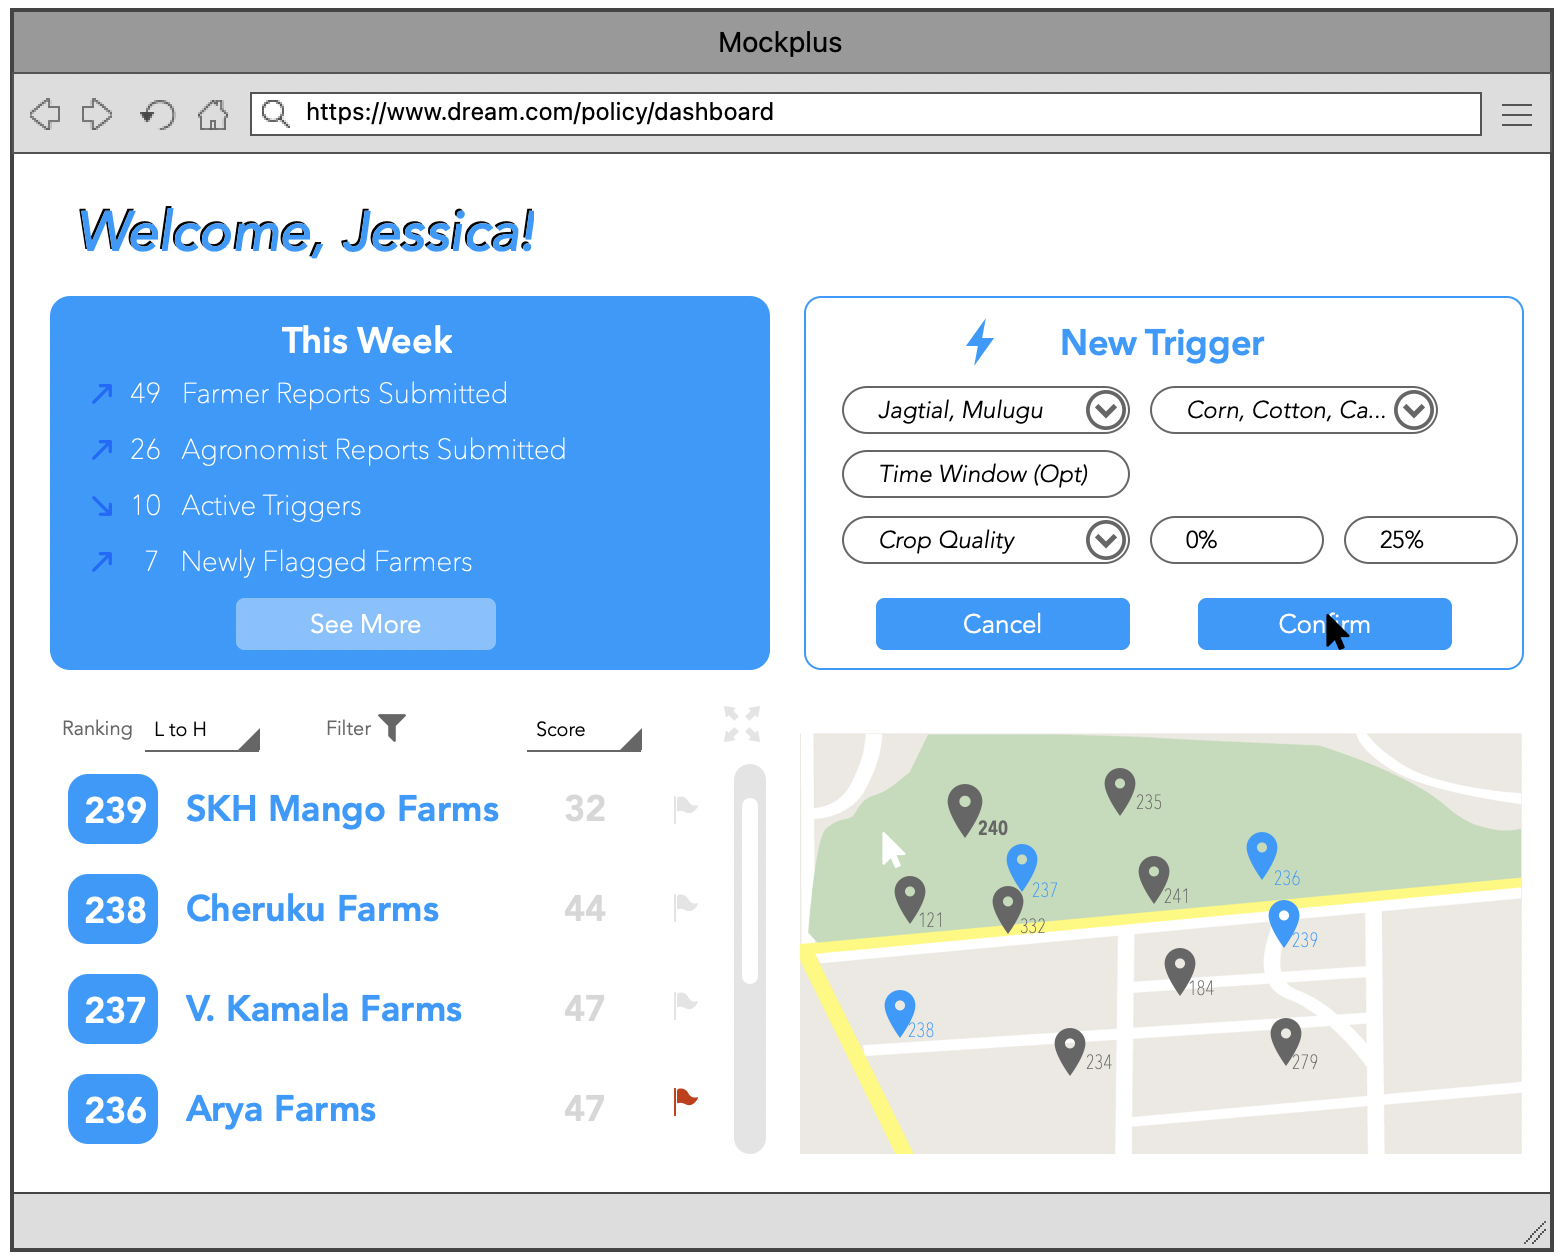
\includegraphics[scale=0.35]{../images_diagrams/mock_ups/dd/Trig05_SetUpDone.png}
\caption{\label{fig:mockpolicy_formComplete}Trigger form complete.}
\end{figure}

\noindent
When the trigger form is submitted, the policy maker can see the newly-added trigger in their Trigger Dashboard. Active triggers can be selected from the policy maker's homepage in order to generate a chart of all the farms eligible for the trigger. From here, the policy maker can see which farmers have satisfied the trigger, and therefore received a flag. From the chart, these farmers are indicated by their data-point being marked as red, whereas in the ranking list-view, these farms are indicated by red flags on the right-hand side.


\begin{figure}[H]
\centering
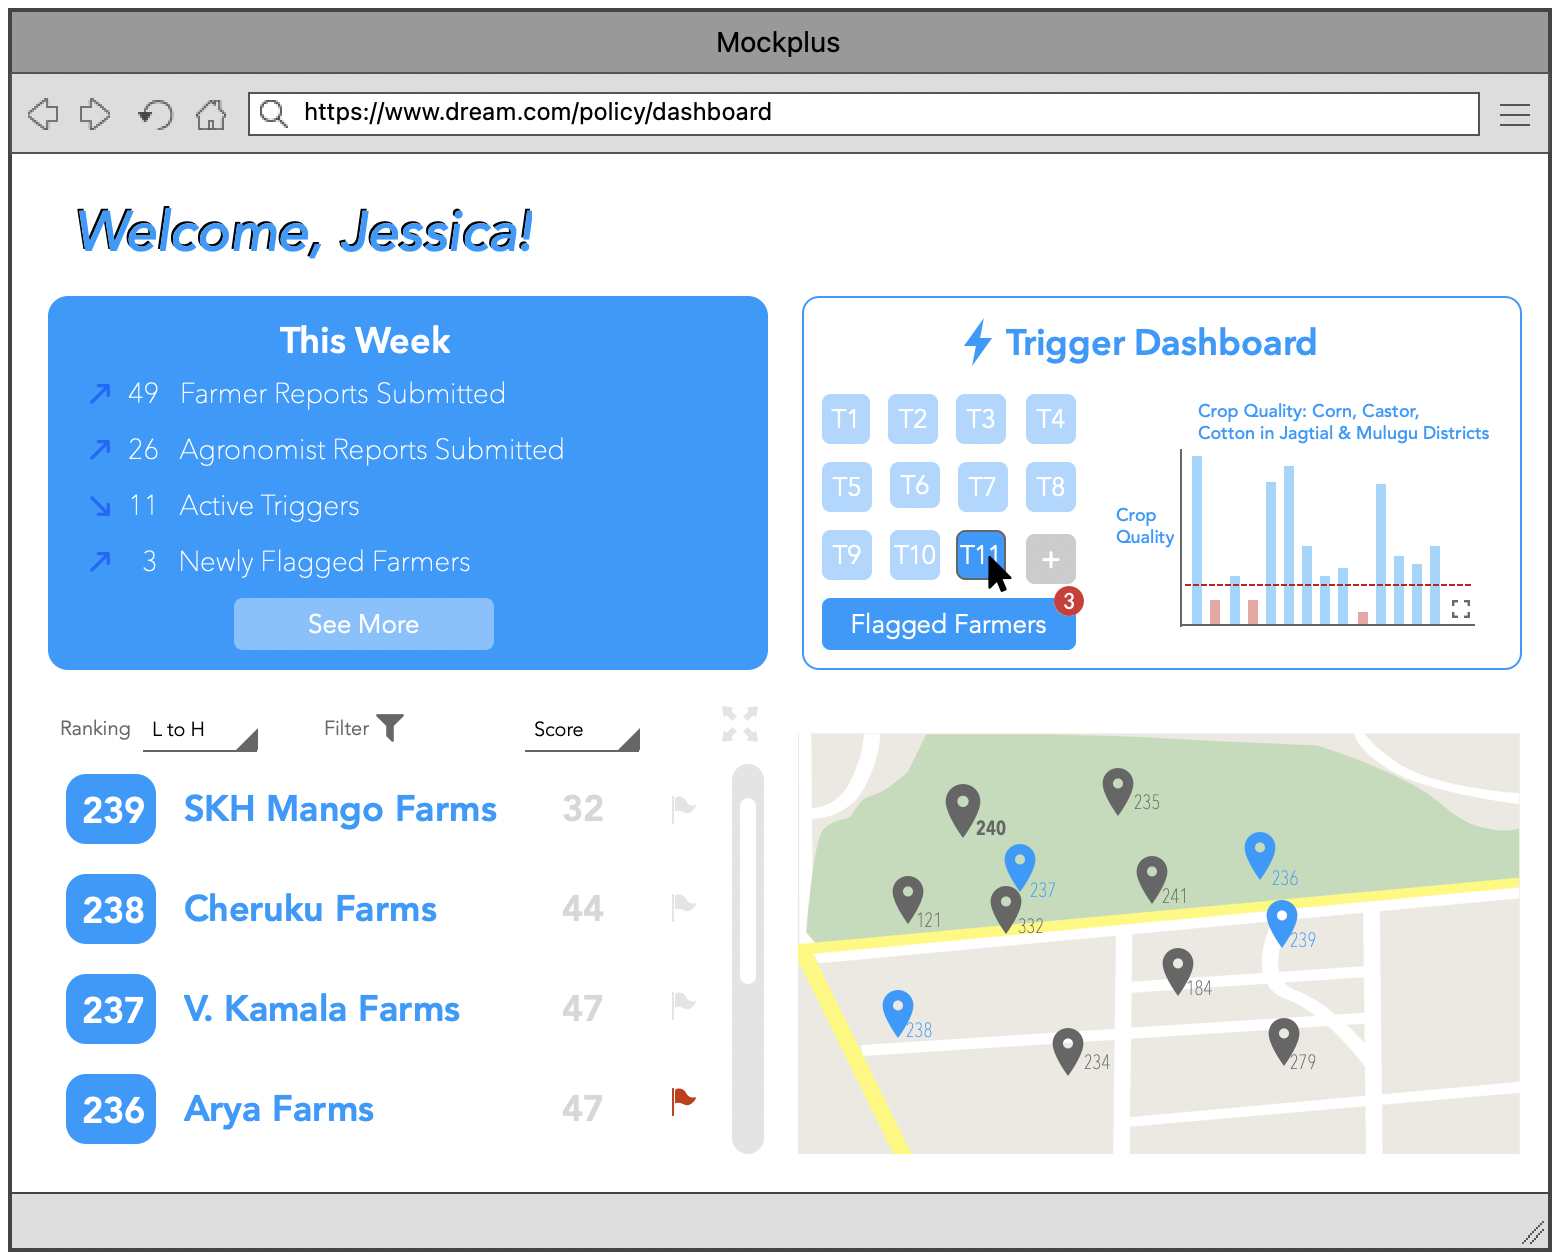
\includegraphics[scale=0.35]{../images_diagrams/mock_ups/dd/Trig06_NewTrigAdded.png}
\caption{\label{fig:mockpolicy_trigEntered}See new trigger from dashboard.}
\end{figure}


